% ============================================================================
%  第 4 章 电磁对偶（原书 pp. 45--60）
%  译自 David Ben-Zvi, "Between Electric-Magnetic Duality and the Langlands Program"
%  Lecture notes by Jackson Van Dyke, UT Austin, Spring 2021.
% ============================================================================
\chapter{电磁对偶}\label{ch:04}

\begin{keytakeaways}
本章把电磁对偶讲成一个可以精确陈述的数学机制。$U(1)$ 规范理论的场空间
$\cC(M)$ 是一个（无穷维）交换 Lie 群，它（非典范地）分裂为格
$\Lambda=H^{2}(M,\Z)$、环面 $T=H^{1}(M,U(1))$ 与向量空间 $V$ 的乘积；把
$F$ 换成 $\star F$ 相当于在这个群上做 Fourier 变换（Pontrjagin 对偶），于是
格（磁通量）与环面（电通量）互换，\emph{'t Hooft} 算子与 Wilson 算子互换。
二维时这退化为 $R\leftrightarrow 1/R$ 的 T-对偶。为了摆脱度量与分析上的困难，
作者随后转入拓扑扭转：把量子力学扩充为 $\mathcal{N}=1,2,4$ 超对称代数，并在
$Q$-上同调中把 Hilbert 空间取成形如 $H^{\bullet}_{U(1)}(\cC(M))$ 的等变上同调。
由此得到 A、B 两类拓扑理论：A-扭转研究 $\mathrm{Pic}(M)$ 的拓扑，B-扭转研究
$\Loc_{\C^{\times}}(M)$ 的代数几何，而电磁对偶恰好交换二者。最后用类时线缺陷与
面缺陷（分歧／螺线管）说明“造磁单极子”与“造电粒子”的对偶。
\end{keytakeaways}

我们此前见过的那些对偶陈述，都只是电磁对偶投下的一个影子。我们将追随
Witten [DEF$^{+}$99]、Freed [Fre00] 以及 Freed--Moore--Segal [FMS07] 的讲法。

\section{经典场论}
\begin{sectionkey}
先在最简单的二维与三维情形里观察对偶的原型：把一个周期标量场 $\varphi$ 的
1-形式 $u=d\varphi$ 换成 $\star u$，方程的形状保持不变，但其几何含义从
“调和映射”变成了“Maxwell 方程”，尺度 $R$ 也变成 $1/R$。
\end{sectionkey}

\subsection{二维}
\label{sec:4-1-1}

我们先研究二维经典场论。设 $\Sigma$ 为黎曼 2-流形。

考虑一个\term{周期标量场}{periodic scalar field}，即一个光滑映射：
\begin{equation}\tag{4.1}
\varphi\in \mathrm{Map}_{C^{\infty}}(\Sigma,S^{1}).
\end{equation}

现在有一个自然的经典场方程要求它满足：\term{调和映射方程}{harmonic map equation}。

方便起见，引入 $\Sigma$ 上的 1-形式 $u=d\varphi$，于是可以写下这组方程：
\begin{equation}\tag{4.2}
\begin{cases}
du=0\\
d\star u=0
\end{cases}.
\end{equation}

第一个方程自动成立，因为 $u$ 已经是恰当形式。第二个方程等价于
$\star d\star u=0$，而这又等价于 $\varphi$ 是调和的。

我们把 (4.2) 写成这种形式，是因为它在 $u\mapsto\star u$ 之下是对称的。换言之，
标量 $\varphi$（满足 $d\varphi=u$）的理论，与某个 $\varphi^{\vee}$（满足
$d\varphi^{\vee}=\star u$）所对应的理论是同一个理论。如果要把度量也纳入考虑，
那么我们研究的是映入某个半径 $R$ 的圆的调和映射，而对偶理论研究的则是映入半径
$1/R$ 的圆的调和映射。这就是 $R\leftrightarrow 1/R$ 对偶。

\begin{srcrem}{16}
对微分形式而言，Poincaré 对偶是由 Hodge 星 $\star$ 实现的，所以我们离之前
所处的地方并不远。
\end{srcrem}

% [Tutor Note: 此处 $\star$ 的归一化约定很关键：$\star\star=\pm1$（黎曼 2-流形上
% 对 1-形式 $\star^{2}=+1$，对 3-维 Lorentz 流形上的 2-形式 $\star^{2}=-1$）。
% 作者在 (4.9) 中取 $B^{\vee}=-\star_{3}E$、在 (4.10) 中取 $E^{\vee}=\star_{3}B$，
% 正是为保证 $(\star F)$ 的分量恰为 $(B^{\vee},E^{\vee})$；若采用相反的 Hodge 星
% 约定，这两个符号会同时反号，$R\leftrightarrow 1/R$ 的结论不变。]

\subsection{三维}
\label{sec:4-1-2}

在三维情形可以玩同样的把戏。设 $\varphi\in \mathrm{Map}_{C^{\infty}}(\Sigma,S^{1})$
为标量场，并令 $u=d\varphi$。我们再次把调和映射方程写成这个漂亮的形式：
\begin{equation}\tag{4.3}
\begin{cases}
du=0\\
d\star u=0
\end{cases}.
\end{equation}

% [Tutor Note: 原文这一段的定义域仍写作 $\Sigma$，但本小节标题与上下文都是三维，
% 因此这里应理解为 3-流形 $M^{3}$；照原样保留记号 $\Sigma$，读者按 $M^{3}$ 理解即可。]

现在从 $u$ 过渡到 $\star u$，是从 1-形式过渡到 2-形式，所以它甚至不再是同一类
对象了。记 $F=\star u$。局部上可以写成
\begin{equation}\tag{4.4}
F=dA
\end{equation}
其中 $A$ 是某个 1-形式，于是我们得到方程
\begin{equation}\tag{4.5}
\begin{cases}
dF=0\\
d\star F=0
\end{cases},
\end{equation}
这正是三维 Maxwell 方程。因此标量场 $\varphi$ 的理论对偶于一个满足 Maxwell
方程的场 $F$ 的理论。

\section{四维／Maxwell 理论入门}
\begin{sectionkey}
在四维 Minkowski 空间中把电场 $E$ 与磁场 $B$ 组装成场强
$F=B-dt\wedge E$，则真空 Maxwell 方程在 $F\leftrightarrow\star F$ 下对称，
这给出 $E\leftrightarrow B$ 的对偶；有源情形下电、磁流的引入会破坏这一对称，
而势 $A$ 的存在（$F=dA$）正是破坏的来源，它导致 Dirac 电荷量子化与
Bohm--Aharonov 效应。
\end{sectionkey}

\term{电场}{electric field}是一个 1-形式 $E\in\Omega^{1}(\R^{3})$，
\term{磁场}{magnetic field}是一个 2-形式 $B\in\Omega^{2}(\R^{3})$。
从相对论的角度看，更好的做法是考虑一个复合的对象，称为\term{场强}{field strength}：
\begin{equation}\tag{4.6}
F=B-dt\wedge E\in\Omega^{2}(M^{4}).
\end{equation}
其中 $M^{4}$ 是 Minkowski 空间。也就是说，我们需要把 $E$ 变成 2-形式，于是用
时间来楔它，这样才能从 $B$ 中把它减掉。

真空中的 Maxwell 方程是：
\begin{equation}\tag{4.7}
\begin{cases}
dF=0\\
d\star F=0
\end{cases}.
\end{equation}
注意它在交换 $F$ 与 $\star F$ 之下是对称的。一些代数运算表明：
\begin{equation}\tag{4.8}
\star F=B^{\vee}-dt\wedge E^{\vee},
\end{equation}
其中 $B^{\vee}$ 是 $E$ 的三维 Hodge 星：
\begin{equation}\tag{4.9}
B^{\vee}=-\star_{3}E,
\end{equation}
类似地
\begin{equation}\tag{4.10}
E^{\vee}=\star_{3}B.
\end{equation}
结论就是：Maxwell 方程在交换 $E$ 与 $B$ 之下是对称的。

如果不在真空中，即存在某些流，那么 Maxwell 方程变成：
\begin{equation}\tag{4.11}
\begin{cases}
dF=j_{B}\\
d\star F=j_{E}
\end{cases}
\end{equation}
其中 $j_{B}$ 是\term{磁流}{magnetic current}，$j_{E}$ 是\term{电流}{electric current}。
它们是 3-形式 $j_{B},j_{E}\in\Omega^{3}(M^{4})$。

这些流的含义在于它们与总电荷有关：
\begin{equation}\tag{4.12}
\int_{M^{3}}j_{B}=Q_{B},
\qquad
\int_{M^{3}}j_{E}=Q_{E},
\end{equation}
这里取 $M^{4}=M^{3}\times\R$。若使用 Stokes 定理，就得到 Gauss 定律。它说：
对闭曲面 $\Sigma\subset M^{3}$，磁通量可以表示为
\begin{equation}\tag{4.13}
b_{\sigma}=\int_{\Sigma}F=\#\,Q_{B,\Sigma}
\end{equation}
其中 $\#$ 是某个标量，$Q_{B,\Sigma}$ 是 $\Sigma$ 内的总磁荷。类似地，电通量为
\begin{equation}\tag{4.14}
e_{\Sigma}=\int_{\Sigma}\star F=\#\,Q_{E,\Sigma}.
\end{equation}

% [Tutor Note: (4.13)、(4.14) 右端的 “$\#$” 是作者留的占位符，原书从未给出它
% 的具体数值。按 Gauss 单位制，$b_{\Sigma}=\int_{\Sigma}F=4\pi Q_{B,\Sigma}$，
% 即在 SI 有理化单位制之外出现 $4\pi$ 因子；这说明这里的 $\#$ 实际是与单位制
% 约定有关的常数（例如 $4\pi$），而不是数学上的未知量。]
% [Tutor Note: (4.13) 左边下标误作 $\sigma$（应随右端作 $\Sigma$），而 (4.19)
% 中积分域写作 $\sigma$、右端又保留未展开的 \texttt{[Sigma]}，这三处是同一处
% 排版疏漏；译文按原样保留 $\sigma$ 并在 (4.19) 处以 $[\Sigma]$ 呈现。]

如果你学过电磁学，大概记得 (4.13) 的右端是 0。这是因为现实中似乎不存在任何
磁单极子，即 $Q_{B}=0$，于是 Gauss 定律说 $\int_{\Sigma}F=0$。正是由于这一性质，
我们可以引入电磁势 $A$，写成：
\begin{equation}\tag{4.15}
F=dA.
\end{equation}
注意这在电与磁之间破坏了对称性，因为 $dF=0$ 现在自动成立。特别地，这意味着
$j_{B}=0$。回忆我们应当考虑
\begin{equation}\tag{4.16}
\nabla=d+A,
\end{equation}
把它看作 $M$ 上某个 $U(1)$-丛上的联络。

场强 $F$ 是有意义的东西，但势 $A$ 带有某种含混性，因为它是 $F$ 的某种原函数。
这种含混性由\term{规范变换}{gauge transformation}
\begin{equation}\tag{4.17}
\nabla\rightsquigarrow g^{-1}\nabla g
\end{equation}
刻画，其中 $g\colon M\to U(1)$。类似地
\begin{equation}\tag{4.18}
A\mapsto A+g^{-1}dg,
\end{equation}
也就是说，$A$ 被平移了某个导数，而这不影响 $F$。

事实上，这是可以被实验测量到的。它称为 \term{Bohm--Aharonov 效应}{Bohm--Aharonov effect}。
即使 $F=0$（平坦联络，即 $E=0$、$B=0$），这个联络的单值性仍是可观测的：
带电粒子沿环路运动时会获得一个相位。

现在可以把这一切设想成任意定向黎曼 4-流形上的联络。当我们从 $F$ 过渡到
$\nabla=d+A$ 时，就实现了 \term{Dirac 电荷量子化}{Dirac charge quantization}，
它大致是说，基本粒子的电荷必须是整数值（在某个重整化之后）。令
$M^{4}=M^{3}\times\R$。于是 $\nabla$ 现在是某个任意线丛 $L$ 上的联络，而
$F$ 和之前一样是 2-形式。即使没有带电粒子，我们仍然有通量：
\begin{equation}\tag{4.19}
b_{\Sigma}=\frac{1}{2\pi i}\int_{\sigma}F=\langle c_{1}(L),[\Sigma]\rangle
\end{equation}
这是 $H^{2}$ 与 $H_{2}$ 之间的配对，因为
\begin{equation}\tag{4.20}
c_{1}(L)\in H^{2}(M,\Z),\qquad [\Sigma]\in H_{2}(M,\Z)
\end{equation}
其中 $\Sigma\subset M^{3}$ 是闭曲面。类似地
\begin{equation}\tag{4.21}
e_{\Sigma}=\int_{\Sigma}\star F.
\end{equation}

% [Tutor Note: (4.20) 原文第二行印作 “$[\Sigma](L)\in H_{2}(M,\Z)$”，多出的
% “$(L)$” 显然是笔误：$[\Sigma]$ 是曲面 $\Sigma$ 的基本类，与线丛 $L$ 无关。
% 译文已按数学含义排为 $[\Sigma]$，并在批注中保留原文痕迹。]
% [Tutor Note: (4.19) 中 $\frac{1}{2\pi i}\int F$ 取值为整数，正是第一 Chern
% 类的 de Rham 代表；这里 $F$ 的归一化（$U(1)$ 的生成元取 $2\pi i\mathbb{Z}$）
% 决定了 Dirac 量子化条件，与 (4.9) 的 Hodge 星符号约定相互独立。]

\section{量子场论}
\begin{sectionkey}
在 Hamilton 形式中，$M^{d-1}\times\R$ 上的量子场论被看成 $M^{d-1}$ 上场空间上的
量子力学。对 Maxwell 理论，Hilbert 空间粗略地就是 $L^{2}(\cC(M^{3}))$；$\cC(M)$
是交换 Lie 群，其分层 $\Lambda\times T\times V$ 给出磁通量的格与电通量的环面，
这为下一节的 Pontrjagin 对偶搭好舞台。
\end{sectionkey}

我们将采用 Hamilton 形式。粗略地说，$M^{d-1}\times\R$ 上的\term{量子场论}{quantum field theory}（QFT）
（把 $M^{d-1}\times\R$ 想成空间乘时间）将是 $M^{3}$ 上某个场空间上的量子力学。
于是我们研究附着在固定时间切片上的 Hilbert 空间，它粗略地是
\begin{equation}\tag{4.22}
L^{2}\bigl(M^{d-1}\text{ 上的场}\bigr).
\end{equation}

% [Tutor Note: 原文这里把空间维数在 $M^{d-1}$ 与 $M^{3}$ 之间来回切换：若
% 时空是 $M^{d-1}\times\R$，则时间切片应是 $M^{d-1}$ 而非 $M^{3}$；下一段的
% (4.23) 又回到 $M^{3}$（此时 $d=4$）。这是讲义随写随改留下的记号不一致，
% 不影响结论，阅读时统一取 $d=4$ 即可。]

在电磁学中，我们从场强 $F$ 出发，然后把它替换成这个联络 $A$。按照上面的启发，
这意味着在 Maxwell 理论中，Hilbert 空间粗略地是
\begin{equation}\tag{4.23}
\cH=\text{“}L^{2}\text{”}\bigl(\cC(M^{3})\bigr)
\end{equation}
其中 $\cC$ 记录线丛 $L$ 与 $U(1)$ 联络 $\nabla$ 的同构类。也就是说，它由联络的
同构类 $|\mathrm{conn}(M)|$ 组成。联络总是有自同构的（至少有圆上的旋转），
但我们只看同构类的集合。

有必要指出，$\cC(M)$ 是一个（无穷维）交换 Lie 群，群运算由张量积给出。交换
Lie 群都形如
\begin{equation}\tag{4.24}
\Lambda\times T\times V
\end{equation}
其中 $\Lambda$ 是某个有限格，$T$ 是某个有限维环面，$V$ 是某个无穷维向量空间。
我们会或多或少忽略 $V$。基本的想法是：对偶两边同时出现格与环面。

现在我们遵循 [FMS07]。可以取第一 Chern 类（底层线丛的同构类）
\begin{equation}\tag{4.25}
\cC(M)\xrightarrow{\ c_{1}\ }H^{2}(M,\Z).
\end{equation}
格就是从这里来的。这是\emph{总}磁通量，其含义是：与曲面配对时，我们得到穿过
该曲面的通量。我们也可以取曲率
\begin{equation}\tag{4.26}
\cC(M)\xrightarrow{\ F\ }\Omega^{2}_{\Z}(M).
\end{equation}
整系数微分形式与整系数的 $H^{2}$ “对话”，于是我们有一个短正合列：
\begin{equation}\tag{4.27}
\begin{array}{ccccccc}
0 & \longrightarrow & \Omega^{1}(M)/\Omega^{1}_{\Z}(M) & \longrightarrow & \cC(M) & \xrightarrow{\ c_{1}\ } & H^{2}(M,\Z)\longrightarrow 0\\[8pt]
 & & \Big\uparrow & & & & \Big\uparrow\\[4pt]
0 & \longrightarrow & \cC_{\mathrm{flat}}(M) & \longrightarrow & \cC(M) & \xrightarrow{\ F\ } & \Omega^{2}_{\Z}(M)\longrightarrow 0
\end{array}
\end{equation}
其中
\begin{equation}\tag{4.28}
\cC_{\mathrm{flat}}(M)=|\Loc_{U(1)}M|=H^{1}(M,\R/\Z)=U(1)\otimes_{\Z}H^{1}(M,\Z)
\end{equation}
是维数为 $b_{1}(M)$ 的环面。有一个映射
\begin{equation}\tag{4.29}
\cC(M)\to\Lambda=H^{2}(M,\Z)
\end{equation}
指向磁通量，而在它的内部有一个环面：
\begin{equation}\tag{4.30}
T=|\Loc_{U(1)}M|\to\cC(M).
\end{equation}

% [Tutor Note: (4.27) 的两个短正合列本来在书中以交换图排版（竖直箭头连接
% $\Omega^{1}/\Omega^{1}_{\Z}$ 与 $\cC_{\mathrm{flat}}$、以及 $H^{2}$ 与
% $\Omega^{2}_{\Z}$）；这里用 \texttt{array} 重排，箭头的连接关系与原图一致。
% 关键点是右端：$H^{2}(M,\Z)$ 与 $\Omega^{2}_{\Z}(M)$ 之间的竖直箭头表示
% “整系数形式的上同调类”这一比较映射，而非 Chern 类映射。]

现在我们将看到，电磁对偶恰好对应于 $\cC(M)$ 上的 Pontrjagin 对偶。我们将能够
用两种方式写出同一个 Hilbert 空间，并且在某种意义上，一边的磁场测量对偶于
另一边的电场测量。

\section{量子场论}
\begin{sectionkey}
本节给出 Lagrangian 形式的示意性框架：对配边 $M$，路径积分
$e^{-S(\varphi)/\hbar}\mathcal{D}\varphi$ 定义一个从 $\cF(\partial M_{\mathrm{in}})$
上的函数到 $\cF(\partial M_{\mathrm{out}})$ 上函数的积分变换 $Z(M)$，它就是
时间演化算子；这正是把拓扑场论的“配边 $\Rightarrow$ 算子”翻译成分析语言的地方。
\end{sectionkey}

\subsection{Lagrangian 形式}
\label{sec:4-4-1}

\begin{flushright}\small 〔课次过渡〕第 7 讲；2021 年 2 月 9 日\end{flushright}

我们将做 $d$ 维的欧氏量子场论。首先给出 Lagrangian 形式的示意性概览。想法是：
对 $d$-流形 $M$，我们附着上一个\term{场空间}{space of fields} $\cF(M)$。
这些是我们空间上的某些局部量，例如函数或丛的截面。

对任意场 $\varphi\in\cF(M)$，可以附着上\term{作用量}{action} $S(\varphi)\in\C$。
这是规定经典运动方程的一种方式。与其去解某个运动方程，不如研究这个函数 $S$
的临界点。

在量子场论中，我们在 $\cF(M)$ 上做某种“概率论”，其“测度”由下式给出：
\begin{equation}\tag{4.31}
e^{-S(\varphi)/\hbar}\mathcal{D}\varphi.
\end{equation}
可以把这东西想成状态空间上的一个“原味”测度，然后被作用量 $S$ 加权。想法是：
当 $\hbar\to0$ 时，它集中到运动方程的解上。我们并不打算让它在数学上严格化，
这只是示意。

对闭的 $M^{d}$，可以附着上\term{配分函数}{partition function}，即这个场空间的
体积（总测度）：
\begin{equation}\tag{4.32}
Z(M)=\int_{\cF(M)}e^{-S(\varphi)/\hbar}\mathcal{D}\varphi.
\end{equation}
这并不是一个很有趣的量，我们常常通过归一化使它等于 1。更有趣的计算对象是
算子的期望值。

\begin{srcex}{25}
算子（具体说，$x\in M$ 处的\term{局部算子}{local operator} $\mathcal{O}_{x}$）
的一个例子，是由在 $x\in M$ 处取值（做一次测量）所给出的 $\cF(M)$ 上的泛函。
\end{srcex}

现在可以取这次测量的期望值：
\begin{equation}\tag{4.33}
\langle \mathcal{O}_{x}\rangle=\frac{\displaystyle\int_{\cF(M)}\mathcal{O}_{x}(\varphi)\,e^{-S(\varphi)/\hbar}\mathcal{D}\varphi}{Z(M)},
\end{equation}
其中我们除以 $Z(M)$ 来归一化测度。接着我们还可以计算\term{关联函数}{correlation function}，
即在不同点做若干次不同测量。

还有“无序”算子：插入这种算子意味着我们去看在 $x$ 处具有指定奇点的场。也就是说，
我们考虑所有场 $\cF(M\setminus\{x\})$，而该算子大致是某个指定奇点空间上的 delta
函数，即它挑出在 $x$ 处具有某种指定奇点的那些场。

% [Tutor Note: “无序算子”与下一段的“有序算子”相对：有序（local）算子作用在
% 场空间上的泛函上，而无序（disorder）算子改变所考虑的场空间本身（引入奇点）。
% 这一区分在第 4.5.1 节会以 't Hooft 算子（改变 $c_{1}$，即无序型）与 Wilson
% 算子（依赖联络，即有序型）的形式再次出现，务必对照阅读。]

\subsection{时间演化}
\label{sec:4-4-2}

设 $M$ 是带边黎曼流形：
\begin{equation}\tag{4.34}
\partial M=\partial M_{\mathrm{in}}\sqcup\partial M_{\mathrm{out}}.
\end{equation}
这是从 $\partial M_{\mathrm{in}}$ 到 $\partial M_{\mathrm{out}}$ 的一个黎曼
\term{配边}{bordism}。图 \ref{fig:4-1} 给出了图示。

\begin{srcex}{26}
设 $N$ 是 $(n-1)$-流形。则 $M=N\times I$ 是从 $N$ 到自身的 $d$ 维配边。
\end{srcex}

% [Tutor Note: 例 26 中若 $N$ 是 $(n-1)$-流形，则 $N\times I$ 应是 $n$ 维配边；
% 原文写作 $d$ 维，是 $n$ 与 $d$ 记号的混用（本段讨论一般的 $d$ 维理论，但
% 例子取的是 $d=n$）。]

\begin{figure}[htbp]
  \centering
  
\includegraphics[width=0.55\textwidth]{figure4-1.png}
  \caption{从两个 $S^{1}$ 的无交并到单个 $S^{1}$ 的配边。（原文 p.~50，Figure 4.1）}
  \label{fig:4-1}
\end{figure}

这给出场的一个对应：
\begin{equation}\tag{4.35}
\begin{array}{cc}
\multicolumn{2}{c}{\cF(M)}\\[4pt]
\swarrow & \searrow\\[2pt]
\cF(\partial M_{\mathrm{in}}) & \cF(\partial M_{\mathrm{out}})
\end{array}
\end{equation}

% [Tutor Note: (4.35) 原书是一个交换图：$\cF(M)$ 在上，两条斜箭头分别指向
% $\cF(\partial M_{\mathrm{in}})$ 与 $\cF(\partial M_{\mathrm{out}})$。这里用
% \texttt{array} 重排，保留原编号；箭头方向与原图一致（都是“限制到边界”）。]

泛函 $e^{-S(\varphi)/\hbar}\mathcal{D}\varphi$ 生活于 $\cF(M)$ 之上，于是我们
得到一个积分变换：先拉回，乘以这个泛函，再积分（推出）。

这个积分变换给出 $\cH_{\mathrm{in}}$ 与 $\cH_{\mathrm{out}}$ 之间的算子 $Z(M)$，
其中
\begin{equation}\tag{4.36}
\cH_{\mathrm{in}}=\text{$\cF(\partial_{\mathrm{in}})$ 上的泛函},
\end{equation}
而
\begin{equation}\tag{4.37}
\cH_{\mathrm{out}}=\text{$\cF(\partial_{\mathrm{out}})$ 上的泛函}.
\end{equation}
于是
\begin{equation*}
\bigl(Z(M)(f)\bigr)(\varphi_{\mathrm{out}})
=\int_{\varphi|_{\partial \mathrm{out}}=\varphi_{\mathrm{out}}}f(\varphi|_{\partial \mathrm{in}})\,e^{-S(\varphi)/\hbar}\mathcal{D}\varphi
=\pi_{\mathrm{out}*}\Bigl(\pi^{*}_{\mathrm{in}}(f)\,e^{-S(\varphi)/\hbar}\mathcal{D}\varphi\Bigr).
\end{equation*}
这个算子就是\term{时间演化算子}{time evolution operator}。

\begin{srcrem}{17}（Hamilton 形式与 Lagrangian 形式）
在 Hamilton 形式中，我们从 Hilbert 空间 $\cH$ 出发，它附着在一个时间切片上。
然后还应当给出一个 Hamilton 算子 $H$，此时时间演化由算子 $e^{iTH/\hbar}$ 给出。
之后我们有一个可观测量的代数，并做各种测量。

另一方面，在 Lagrangian 形式中，我们从场空间与作用量出发。Lagrangian 表述非常
灵活，因为它允许我们定义这些推出—拉回算子，而 Hamilton 形式中的 Hilbert 空间
与时间演化算子（即 Hamilton 量）正是由此恢复出来的。
\end{srcrem}

\begin{srcex}{27}
一维量子场论就是量子力学。设 $X$ 是黎曼靶空间。那么场空间可能是
$\cF(\R)=\mathrm{Maps}(\R,X)$。$S$ 的临界点将是 $X$ 中的测地线。Hilbert 空间是
\begin{equation}\tag{4.38}
\cH=L^{2}(\mathrm{Maps}(\mathrm{pt},X))=L^{2}(X),
\end{equation}
而 Hamilton 量是 Laplace 算子 $\Delta$。
\end{srcex}

要把这一切严格化需要大量的工作。我们也不想使用任何微扰技术，因为我们并不
一定希望 $\hbar$ 很小。我们将把它当作示意性的指南，并形式地过渡到拓扑情形。

\section{量子 Maxwell 理论}
\begin{sectionkey}
四维 $U(1)$ 规范理论的经典作用量由 Yang--Mills 项与拓扑项
$\theta\int F\wedge F$ 组成；在 $M^{4}=M^{3}\times\R$ 上，Hilbert 空间是
$L^{2}(\cC(M^{3}))$，而 $\cC(M^{3})$ 按 $\Lambda=H^{2}(M,\Z)$、平坦联络环面 $T$
与向量空间 $V$ 分裂。't Hooft 算子实现 $\Lambda$ 的平移，Wilson 算子实现 $T$ 的
特征，二者分别对应磁与电的测量。
\end{sectionkey}

我们考虑一个四维量子场论。$4$-流形 $M^{4}$ 上的场空间由带联络 $d+A$ 的
$U(1)$-丛组成（$A$ 是电磁势），模去规范等价，即模去规范变换的作用。

经典运动方程是 Maxwell 方程：
\begin{equation}\tag{4.39}
\begin{cases}
dF=0\\
d\star F=0
\end{cases},
\end{equation}
其中 $F$ 是曲率。于是我们得到作用量
\begin{equation}\tag{4.40}
S=\frac{g}{2\pi i}\int_{M}F\wedge\star F+\theta\int_{M}F\wedge F.
\end{equation}

第二项中的积分只是在计算线丛的 $c_{1}^{2}=p_{1}$。这一项
\footnote{原文此处有旁注：“constants?”（是常数吗？）。}被称为\term{拓扑项}{topological term}。

% [Tutor Note: (4.40) 的归一化是 Maxwell 理论中最容易搞混的地方。通常写
% $S=\frac{1}{4e^{2}}\int F\wedge\star F+\frac{i\theta}{8\pi^{2}}\int F\wedge F$；
% 作者把 Yang--Mills 系数记成 $\frac{g}{2\pi i}$、把拓扑项系数记成 $\theta$，
% 这只是把 $g,\theta$ 吸收进定义。要点是：$\int F\wedge F$ 只依赖线丛的同构类，
% 因而在连续形变下不变（这就是它被称为“拓扑项”的原因）；在 $U(1)$ 情形它等于
% $c_{1}^{2}=p_{1}$ 的积分，取整数值，故 $\theta$ 以 $2\pi$ 为周期。]

想法是：Hilbert 空间附着在一个特定的时间切片上。于是假设可以写成
$M^{4}=M^{3}\times\R$，此时 Hilbert 空间是
\begin{equation}\tag{4.41}
\cH=L^{2}\bigl(\cC(M^{3})\bigr)
\end{equation}
其中 $\cC(M^{3})$ 表示 $M^{3}$ 上带联络的线丛模规范变换所得的集合。
$\cC(M^{3})$ 是一个交换 Lie 群，并且有一个到可能线丛同构类的格的映射：
\begin{equation}\tag{4.42}
\cC(M^{3})\xrightarrow{\ c_{1}\ }\Lambda=H^{2}(M,\Z),
\end{equation}
此外它还有一个由平坦联络构成的子环面：
\begin{equation}\tag{4.43}
T=\{\text{平坦联络}\}\simeq H^{1}(M,\R/\Z=U(1))\simeq BH^{1}(M,\Z)\to\cC(M^{3}),
\end{equation}
其中 $U(1)$ 取离散拓扑。于是 $\cH$ 的最后一个因子由一个无穷维向量空间 $V$
给出。也就是说，存在一个（非典范的）分裂 $\cC(M)\simeq\Lambda\times T\times V$。

% [Tutor Note: (4.43) 中出现的 “$BH^{1}(M,\Z)$” 在书中没有定义，$B$ 记号很
% 可能是笔误或作者自己的速记。数学上应读作 $T\simeq\Hom(H_{1}(M),\R/\Z)
% \simeq H^{1}(M,\Z)\otimes_{\Z}\R/\Z$；若坚持 $U(1)$ 取离散拓扑，则 $T$ 成为
% 一个无穷离散群，“环面”的说法只在通常拓扑下成立。]

\subsection{算子}
\label{sec:4-5-1}

现在我们要在 $\cH$ 上辨认出一些从这套设定中自然出现的算子（即可观测量）。
首先要说的是，$\cH$ 有一个由 $\Lambda=H^{2}(M,\Z)$ 给出的显然分次。这已经挑出了
一些算子，例如告诉你处在哪个连通分支上。这就是磁通量，所以说这是按磁通量的
分次。

\subsection*{Dirac／'t Hooft 算子}

$\Lambda$ 也作用在 $\cH$ 上，给出 \emph{'t Hooft 算子}。
\footnote{严格说来，'t Hooft 算子是这些东西的非阿贝尔推广。这些算子实际上与
Dirac 单极子有关，但“Dirac 算子”一词早已另有含义，那样叫会造成混淆。}
如果已经选定了分裂 $\cC(M)\simeq\Lambda\times T\times V$，那么这个作用就只是平移。
也就是说，这些算子平移磁通量。回忆通量大致记录了所包围的单极子数目。所以
物理上这些算子产生磁单极子。

更精确地说，设 $\gamma$ 是 $M$ 中的简单闭曲线。注意它定义了一个类
\begin{equation}\tag{4.44}
[\gamma]\in H_{1}(M,\Z)\simeq H^{2}(M,\Z)\simeq\Lambda.
\end{equation}
相应的算子如下所述地沿 $\gamma$ 引入一个单极子。想法是：$\gamma$ 位于
$M^{3}\times I$ 中某个特定的时间切片上，而我们研究的是 $M\times I$ 上沿
$\gamma$ 带一个单极子的电磁学，如图 \ref{fig:4-2}。

换言之，我们考虑场 $\cC(M\times I\setminus\gamma)$，即联络可能沿 $\gamma$ 有
奇点。于是我们把这个纽结挖去，这在我们的 4-流形上引入了一个新的边界分支：
纽结的环绕（纽结管状邻域的边界），它看起来像 $S^{2}\times S^{1}$。然后我们可以
考虑在这个边界上具有特定积分的联络。特别地，我们可以要求
\begin{equation}\tag{4.45}
\frac{1}{2\pi i}\int_{S^{2}}F=1.
\end{equation}
把所得的场空间记作
\begin{equation}\tag{4.46}
\cC(M\times I\setminus\gamma)_{c_{1}=1}.
\end{equation}
注意，物理上这就是说曲面 $S^{2}\times S^{1}\subset M^{3}\times I$ 包含磁荷 1。
数学上我们看到的是：我们无法把这个联络延拓过这条曲线。物理上我们看到的是
沿着这条曲线的一个单极子。

\begin{figure}[htbp]
  \centering
  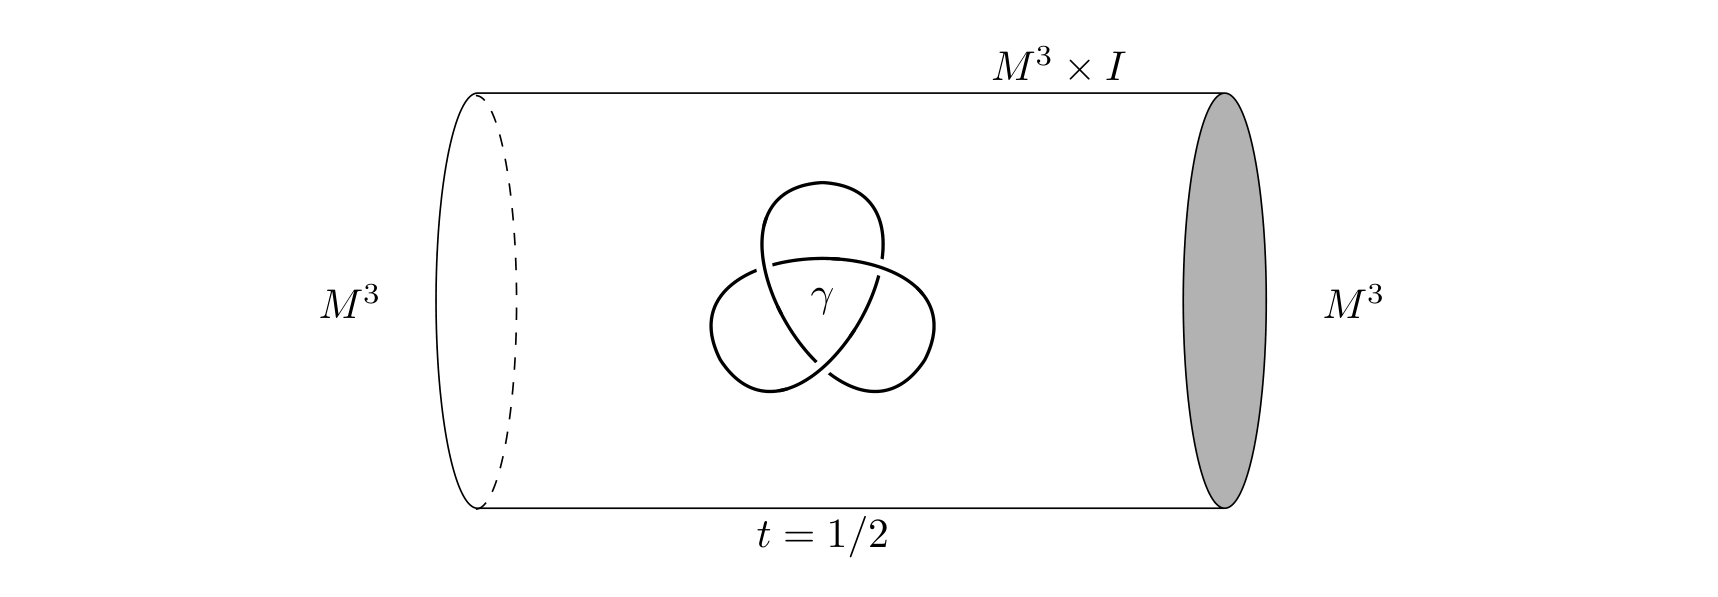
\includegraphics[width=0.55\textwidth]{figure4-2.png}
  \caption{环路 $\gamma$ 位于 $M^{3}\times I$ 的某个时间切片中，比如 $t=1/2$。
  我们可以把它挖去，所得 4-流形上的场可能沿 $\gamma$ 出现奇点；要求绕 $\gamma$
  的一个邻域的边界积分等于 1，便给出 $\gamma$ 邻域内部具有受控奇点的场空间。
  物理上这沿着 $\gamma$ 引入一个磁单极子。（原文 p.~52，Figure 4.2）}
  \label{fig:4-2}
\end{figure}

真正的算子是这样定义的。4-流形 $M\times I\setminus\gamma$ 是从 $M^{3}$ 到自身
的配边，因此像往常一样定义了一个对应与积分变换（Feynman 路径积分）：
\begin{equation}\tag{4.47}
\begin{array}{c}
\begin{array}{ccc}
 & \cC(M\times I\setminus\gamma)_{c_{1}=1} & \\[4pt]
{\scriptstyle\pi_{\mathrm{in}}}\swarrow & & \searrow{\scriptstyle\pi_{\mathrm{out}}}\\[4pt]
\cC\bigl(M^{3}_{\mathrm{in}}\bigr) & & \cC\bigl(M^{3}_{\mathrm{out}}\bigr)
\end{array}\\[10pt]
\cH\xrightarrow{\ \pi_{\mathrm{out}*}\bigl(e^{-S(\varphi)/\hbar}\mathcal{D}\varphi\,\pi^{*}_{\mathrm{in}}(-)\bigr)\ }\cH
\end{array}
\end{equation}
物理上，这个算子把状态空间沿时间演化，在此期间沿 $\gamma$ 引入一个单极子，
然后再把它移除。数学上它把 Chern 类平移 $[\gamma]$，也就是说，它只是与一个
具有指定 Chern 类的平坦线丛做张量积
\begin{equation}\tag{4.48}
c_{1}=[\gamma]\in H^{2}(M,\Z).
\end{equation}

% [Tutor Note: (4.47) 的交换图在原文中由“顶空间 + 两个投影 $\pi_{\mathrm{in}},
% \pi_{\mathrm{out}}$ + 底部的两个 $\cH$”构成，底部水平箭头标出的是积分核
% $\pi_{\mathrm{out}*}(e^{-S/\hbar}\mathcal{D}\varphi\,\pi^{*}_{\mathrm{in}}(-))$；
% 这里用 \texttt{array} 重排，保留了全部箭头与编号。“挖去 $\gamma$ 后$c_1=1$”
% 意味着联络在环绕 $S^{2}\times S^{1}$ 上的积分非零，故不能延拓——这正是
% 't Hooft 算子作为“无序算子”的几何含义。]

\subsection*{Wilson 环路算子}

另一方面，还有更简单的可观测量，称为 \term{Wilson 环路算子}{Wilson loop operator}。
仍设 $\gamma\subset M$ 是简单闭曲线。它决定了 $\cC(M)$ 上的一个函数 $W_{\gamma}$：
\begin{equation}\tag{4.49}
W_{\gamma}\colon (\cL,\nabla)\mapsto \text{沿 }\gamma\text{ 的和乐}\in U(1)\subset\C.
\end{equation}
我们可以画与图 \ref{fig:4-2} 同样的图，但我们对它做的事情完全不同。我们仍然把
$\gamma$ 想成位于 $M\times I$ 内某个时间切片上。现在，随着时间演化，我们做沿
$\gamma$ 的和乐测量。所以这与例 25 中局部算子的例子是同一类测量，只不过现在
测量是沿一个环路做的，因此称为线／环算子。这仍然给出一个对应与积分变换，
只不过现在变换的核由函数 $W_{\gamma}$ 给出：
\begin{equation}\tag{4.50}
\begin{array}{c}
\begin{array}{ccc}
 & \cC(M\times I) & \\[4pt]
{\scriptstyle\pi_{\mathrm{in}}}\swarrow & & \searrow{\scriptstyle\pi_{\mathrm{out}}}\\[4pt]
\cC\bigl(M^{3}_{\mathrm{in}}\bigr) & & \cC\bigl(M^{3}_{\mathrm{out}}\bigr)
\end{array}\\[10pt]
\cH\xrightarrow{\ \pi_{\mathrm{out}*}\bigl(W_{\gamma}\,\pi^{*}_{\mathrm{in}}(-)\bigr)\ }\cH
\end{array}
\end{equation}
要点是：我们可以把联络空间上的函数乘以这个函数 $W_{\gamma}$。所以按照我们
呈现 Hilbert 空间的方式，这些 Wilson 算子已经被对角化了。

Wilson 环路 $W_{\gamma}$ 是平坦联络空间作用的本征函数：
\begin{equation}\tag{4.51}
T=\cC_{\flat}(M)\simeq H^{1}(M,U(1)).
\end{equation}
它通过张量积作用在 $\cC(M)$ 上，因此也作用在 $L^{2}(\cC(M))$ 上。本征值由沿
$\gamma$ 的单值性给出：给定一个平坦联络（$H^{1}(M,U(1))$ 的元素），取沿
$\gamma$ 的单值性便典范地得到 $U(1)$ 的一个元素，而这正是在做 Fourier 级数。
这些 $W_{\gamma}$ 就是这个环面 $T$ 的特征。

\subsection{电磁对偶}
\label{sec:4-5-2}

注意，当我们研究 't Hooft 算子时，我们关注的是格的作用，并且有按磁通量的分次。
现在我们关注环面作用，并且可以对角化。这给出按 $T$ 的特征的分解，而这些特征
构成格 $H^{2}(M,\Z)$：
\begin{equation}\tag{4.52}
\cH=\bigoplus_{e\in H^{2}(M,\Z)}\cH_{e},
\end{equation}
这可以解释为按电通量的分次。

从磁分次过渡到电分次，恰好是对场空间的环面部分做 Fourier 变换。一般说来，
电磁对偶可以看成在我们场的 Lie 群上做 Fourier 级数。它具体地识别出
\begin{equation}\tag{4.53}
L^{2}\bigl(\cC_{U(1)}(M)\bigr)\simeq L^{2}\bigl(\cC_{U(1)^{\vee}}(M)\bigr),
\end{equation}
其中左边是 $F$ 侧，右边是 $\star F$ 侧。这个群总是分裂为格、环面与向量空间
（我们忽略最后一个）。$F$ 侧与 $\star F$ 侧分别对应如下分裂：
\begin{equation}\tag{4.54}
\Lambda_{B}\times T_{E}\times\mathrm{Vect}
\qquad\qquad
\Lambda_{E}\times T_{B}\times\mathrm{Vect}.
\end{equation}
$\Lambda_{B}$ 是磁通量的格，$T_{B}$ 是它的对偶环面，$\Lambda_{E}$ 是电通量的格，
$T_{E}$ 是它的对偶环面。在 $F$（左）侧，Wilson 环路算子被对角化；在 $\star F$
（右）侧，'t Hooft 算子被对角化。类似地，磁的 $b$ 分次变成电的 $e$ 分次。

% [Tutor Note: (4.53) 这个“等式”只在忽略向量空间因子 $V$ 的意义下成立：两边
% 的 $L^{2}$ 都含有同一个 $L^{2}(V)$ 因子，作者把它略去。真正的内容是
% Pontrjagin 对偶 $L^{2}(T)\simeq L^{2}(\Lambda^{\vee})$，以及
% $L^{2}(\Lambda)\simeq L^{2}(T^{\vee})$，即 Fourier 变换交换 $\Lambda$ 与 $T$。
% 把 $\Lambda_B\times T_E$ 与 $\Lambda_E\times T_B$ 对照 (4.54)，就能看出
% “$F$ 侧对角化 Wilson、$\star F$ 侧对角化 't Hooft” 的含义。]

\section{二维中的阿贝尔对偶}
\begin{sectionkey}
二维的电磁对偶就是 T-对偶（镜像对称）。场空间
$\mathrm{Map}(S^{1},S^{1}_{R})$ 是交换 Lie 群，Hilbert 空间
$L^{2}$ 的分解按绕数由 $H^{1}(S^{1},\Z)$ 分级；对偶理论以
$R\leftrightarrow1/R$ 的靶空间出现，其分级改由 $H^{0}(S^{1},U(1))$ 给出，
两套算子（'t Hooft 型与 Wilson 型）在对偶下互换。
\end{sectionkey}

回忆这被称为 T-对偶，或镜像对称。场空间是 $\mathrm{Map}(M,S^{1})$，或者更一般地
映入某个环面 $T$。我们在 $S^{1}$ 上的 Hilbert 空间 $\cH$ 于是是
\begin{equation}\tag{4.55}
L^{2}\bigl(\mathrm{Map}(S^{1},S^{1}_{R})\bigr).
\end{equation}
注意 $\mathrm{Map}(S^{1},S^{1})$ 在逐点乘法之下又是一个交换 Lie 群，即我们用
的是靶空间的群结构而非源空间的。这里也有一个到格的映射：它按
$H^{1}(S^{1},\Z)$ 分次，这是通过取绕数给出的。

对偶地，我们可以研究：
\begin{equation}\tag{4.56}
L^{2}\left\langle \mathrm{Maps}\left\langle S^{1},(S^{1}_{R})^{\vee}=S^{1}_{1/R}\right\rangle\right\rangle.
\end{equation}
它按 $H^{0}(S^{1},U(1))$ 分次，与上面的分次对偶。我们有一个由平移绕数给出的
算子（'t Hooft 算子的类似物），以及由在一点取值给出的算子（Wilson 算子的
类似物），而对偶交换它们。

% [Tutor Note: (4.55)--(4.56) 中“$S^{1}_{R}$”表示半径 $R$ 的圆。T-对偶的
% 标准陈述是：半径 $R$ 的圆上的自由玻色子等价于半径 $1/R$（在 $\alpha'=1$
% 的单位下）的圆上的自由玻色子，同时把动量模与绕数模互换。这里的分级
% $H^{1}(S^{1},\Z)=\Z$（绕数）与 $H^{0}(S^{1},U(1))$（取值）正是这一互换的
% 代数表现。原文用双重尖括号 $\langle\langle\cdots\rangle\rangle$ 排版，是一个
% 排版习惯，不影响含义。]

\section{拓扑量子力学／量子场论}
\begin{sectionkey}
量子力学之所以难，是因为要处理分析。Witten 的超对称技巧把
$L^{2}(X)$ 换成微分形式 $\Omega^{\bullet}(X)$，并加入 de Rham 微分 $Q=d$ 与
$Q^{*}=d^{*}$，使得 $H=[Q,Q^{*}]$，于是 $H$ 在 $Q$-上同调上为零：
时间被“导出地”杀死了，剩下的只是 $X$ 的上同调。
\end{sectionkey}

想法是：量子力学之所以难，是因为它涉及分析。在通常的量子力学中，我们从一点
出发，附着上一个 Hilbert 空间 $\cH$。然后对一个长度为 $T$ 的区间，我们附着上
酉时间演化算子
\begin{equation}\tag{4.57}
e^{iTH/\hbar}.
\end{equation}
在\term{拓扑量子力学}{topological quantum mechanics}（TQM）中，我们想杀死时间，
即我们希望 $H=0$。最朴素的解释方式是限制到基态。但闭流形上不存在非常值的
有界调和函数。所以这样一来我们把整个理论都杀死了。

Witten [Wit82] 引入了如下技巧，通过\term{超对称}{supersymmetry}（SUSY）
在导出的意义下杀死时间。设 $X$ 是黎曼流形。我们不用 $L^{2}(X)$，而是把
Hilbert 空间扩充为 $L^{2}$ 微分形式，即我们加入新的场，于是得到一个由超 Lie 群
给出的更大对称群。现在考虑：什么作用在微分形式上？首先是 Laplace 算子
$H=\Delta$。我们还有 de Rham 微分 $Q=d$ 及其伴随 $Q^{*}=d^{*}$。还有一个给出
$\Z$-分次的 $U(1)$ 作用。这套算子称为 $\mathcal{N}=1$ 超对称代数。于是我们有
算子 $H$（次数 0）、$Q$（次数 1）与 $Q^{*}$（次数 $-1$）。这些算子大多交换：
\begin{equation}\tag{4.58}
[Q^{*},Q^{*}]=[Q,Q]=0,
\end{equation}
\begin{equation}\tag{4.59}
[Q,H]=[Q^{*},H]=0,
\end{equation}
除了
\begin{equation}\tag{4.60}
[Q,Q^{*}]=H.
\end{equation}
$[Q,Q]=0$ 可以解释为 $d^{2}=0$。另一个关系是
\begin{equation}\tag{4.61}
\Delta=dd^{*}+d^{*}d,
\end{equation}
它说的是 $Q^{*}$ 给出从 $H$ 到 $0$ 的一个同伦。特别地，这意味着在
$Q$-上同调上，$H$ 的作用为 0。

于是我们加入了新场，得到了更大的对称代数。这个代数中的一个算子是平方为零的
奇算子，我们称之为微分。在相应的上同调上，$H$ 为零。所以我们在导出的意义下
杀死了时间。于是拓扑量子力学给 $X$ 附着上复形
\begin{equation}\tag{4.62}
\bigl(\Omega^{\bullet}(X),d\bigr),
\end{equation}
或者 $H^{*}(X)$。在第一种情形 $H$ 同伦于 0，在后一种情形 $H=0$。这就是从
量子力学中恢复 de Rham 上同调的方式。

% [Tutor Note: 这里“杀死时间”的准确含义是：在 $Q$-上同调（即把 $Q$-恰当形式
% 视为零）中，$H=[Q,Q^{*}]$ 作用为零，于是时间演化 $e^{iTH/\hbar}$ 在同调上
% 变成恒等。注意 $[Q,Q^{*}]=H$ 的符号依赖于 $Q^{*}$ 取 $d^{*}$ 还是 $-d^{*}$；
% 若取 $Q^{*}=-d^{*}$，则右边多一个负号，但“在 $Q$-上同调上 $H=0$”的结论不变。]

我们将永远不处理真正意义上的量子场论。相反，我们要做的是这种拓扑扭转。注意在
这套设定中，理论只拓扑地依赖于 $X$。结论就是：我们正在杀死对黎曼度量的依赖，
这会让日子好过得多。

\begin{flushright}\small 第 8 讲；2021 年 2 月 11 日\end{flushright}

\section{拓扑量子力学}
\begin{sectionkey}
TQM 的两种实现：A-型取 $(\Omega^{\bullet}(X),d)$，得上同调
$H^{\bullet}_{dR}(X)$；B-型取 $(\Omega^{0,\bullet}(X),\bar\partial)$，得
Dolbeault 上同调 $H^{0,*}(X)$。进一步还有 $\mathcal{N}=2$（Kähler 流形，
Lefschetz $\mathrm{SL}_{2}$ 作用）与 $\mathcal{N}=4$（超 Kähler 流形，
$\mathrm{Spin}(5)$ 作用）的版本。
\end{sectionkey}

\begin{flushright}\small 〔课次过渡〕\end{flushright}

形式地建立这套东西的方式是：有一个 $d=1$、$\mathcal{N}=1$ 的超对称代数作用在
$\cH$ 上。$d=1$ 意味着我们在做量子力学，而 $\mathcal{N}=1$ 只是说超对称的量
最少。

TQM 有两种自然的实现。第一种是 \emph{A-型} TQM。取 $X$ 为黎曼流形，那么
Hilbert 空间由微分形式组成：
\begin{equation}\tag{4.63}
\cH=\Omega^{\bullet}(X),
\end{equation}
Hamilton 量 $H=\Delta$ 是 Laplace 算子，$Q=d$ 是 de Rham 微分，而
$Q^{*}=d^{*}$ 是关于度量的伴随。分次是形式上的通常分次，上同调是
\begin{equation}\tag{4.64}
H^{\bullet}(\cH)=H^{\bullet}_{dR}(X).
\end{equation}

还有另一种实现，称为 \emph{B-型} TQM。此时取 $X$ 为复流形。Hilbert 空间是
\begin{equation}\tag{4.65}
\cH=\Omega^{0,\bullet}(X),
\end{equation}
即含 $\bar\partial$ 的形式。SUSY 算子由 $Q=\bar\partial$、$Q^{*}=\bar\partial^{*}$
与 $H=\Delta_{\bar\partial}$ 给出。上同调是 Dolbeault 上同调：
\begin{equation}\tag{4.66}
H^{0}(\cH)=H^{0,*}(X)=R\Gamma(\cO_{X}).
\end{equation}

这两种都是 1 维 $\mathcal{N}=1$ 超对称代数的实现。还有
$\mathcal{N}=2$ TQM。一个这样的例子来自研究 Kähler 流形 $X$。Hilbert 空间
仍然是微分形式：
\begin{equation}\tag{4.67}
\Omega^{\bullet,\bullet}(X).
\end{equation}
它是双分次的，而不像之前那样只有一个分次；它带有一批算子，例如
$\partial$、$\bar\partial$、$\partial^{*}$ 与 $\bar\partial^{*}$。
Kähler 恒等式告诉我们相应的 Laplace 算子相等：$\Delta_{\bar\partial}=\Delta_{d}$。

对数学家而言，有下面这个深刻的定理。我们有一个 $\mathrm{SU}(2)$ 在
$\Omega^{\bullet,\bullet}(X)$ 上的作用，可以把它想成来自复化
$\mathrm{SU}(2)\subset \mathrm{SL}_{2}\C$。这些就是 Lefschetz 算子。对角部分
给出上同调分次，然后有一个提升算子（与 Kähler 形式作交）和一个下降算子。
数学上这是关于 Kähler 流形整体上同调的一个非常深刻的陈述（硬 Lefschetz 定理）。
物理上这是在计算什么样的超对称代数作用在我们的 Hilbert 空间上，而这个
$\mathrm{SU}(2)$ 作用就是 R-对称。要点在于我们找到了一个很大的超对称代数。

$\mathcal{N}=1$ 超对称代数编码了黎曼流形的 Hodge 理论。这个 $\mathcal{N}=2$
超对称代数编码了复 Hodge 理论。还有 $\mathcal{N}=4$ TQM。此时我们研究紧超
Kähler 流形 $X$ 上的微分形式：$\Omega^{\bullet}(X)$。超 Kähler 情形下 Lefschetz
$\mathrm{SL}_{2}$ 作用的类似物是 $\mathrm{Spin}(5)$ 的作用。想法是：若把所有
Lefschetz $\mathrm{SL}_{2}$ 拼在一起，就得到一个 $\mathrm{Spin}(5)$。这是一个
我们不会写下来的超 Lie 群的一部分。从物理的观点看，这只是在研究这个流形上的
粒子理论时，对“周围坐着哪些算子”做的一个自然计算。

\begin{srcrem}{18}
还有 $\mathcal{N}=8$ 超对称。这些不同的超对称代数实际上是按存在的奇算子
（又称超荷 $Q$）的数目来区分的。例如 $\mathcal{N}=1$ 有两个，
$\mathcal{N}=2$ 有四个，$\mathcal{N}=4$ 有八个，而 $\mathcal{N}=8$ 有十六个。
\end{srcrem}

% [Tutor Note: 原文末句作 “$\mathcal{N}=8$ had 16”，时态 “had” 是笔误，
% 应为 “has”。另外“奇算子个数 = $2\mathcal{N}$”这一计数只在
% $\mathcal{N}\le 4$ 时与通常的物理约定一致；对 $\mathcal{N}=8$，超荷通常
% 计入其反粒子共轭，实际独立超荷数会因维数约化约定而不同，阅读时以原文的
% 计数为准即可。]

% [Tutor Note: (4.66) 中 $R\Gamma(\cO_{X})$ 的写法只在 $X$ 紧合（例如射影）
% 时才与 $H^{0,*}(X)$ 同构；一般复流形上应写作 $H^{0,*}_{\bar\partial}(X)$
% 与 $R\Gamma(\cO_X)$ 的导出范畴对象，而不是相等。作者在此处把
% “$H^{0}(\cH)$” 与 Dolbeault 上同调等同，是按紧 Kähler 情形书写的。]

TQM 乃至最终 TQFT 的一般哲学是：加入场，使得有一个大的超 Lie 群（超对称代数）
作用。我们要找两样东西：
\begin{enumerate}
\item Hamilton 量是恰当的：$H=[Q,-]$（即我们杀死了时间\footnote{即时间演化被
变得平凡。}），以及
\item $T=[Q,-]$，即度量依赖是恰当的（即我们杀死了几何）。
\end{enumerate}
\term{能量动量张量}{stress energy tensor} $T$ 是 QFT 中的一个对象，它衡量对
度量的依赖。数学上 $T$ 是等距不变性的导出版本。Costello--Gwilliam [CG17] 中
对此有很好的解释。

\subsection{拓扑 Maxwell 理论}
\label{sec:4-8-1}

我们想取光的量子理论（普通 Maxwell 理论），加入一些场，并找出超对称代数。
然后我们挑一个 $Q$ 并过渡到上同调。这将是一个 $\mathcal{N}=4$ 的 GL-扭转理论。
特别地，这个 $\mathcal{N}=4$ 意味着有大量超对称：将会有十六个超荷。

之前，我们的场空间由一个线丛与一个联络 $\nabla=d+A$ 的选择组成。现在我们要
加入：
\begin{itemize}
\item 流形上的一个 1-形式 $\sigma$（\term{Higgs 场}{Higgs field}），
\item 一个复标量 $u$，以及
\item 四个费米子（奇场）（我们不会太关注它们）。
\end{itemize}
Hilbert 空间原本是 $\cH=L^{2}(\cC(M))$。现在，在 A-扭转中，3-流形 $M^{3}$ 被
附着到这个空间的\emph{上同调}上：$H^{\bullet}(\cC(M))$。我们现在有一个大得多
的场空间，但在上同调层面这其实没有区别，因为引入这些新场并没有改变空间的
拓扑。但结果是：我们不要通常的上同调，我们要的是关于联络自同构等变的上同调，
即我们要的是：
\begin{align}
\cH&=H^{\bullet}(\text{联络}/\text{规范等价})\tag{4.68}\\
&=H^{\bullet}_{U(1)}\bigl(\cC(M)\bigr).\tag{4.69}
\end{align}
这是在联络空间上做 de Rham 意义下的拓扑量子力学。

% [Tutor Note: (4.69) 的下标 $U(1)$ 指对联络的自同构群（每点的 $U(1)$ 旋转，
% 即规范变换）取等变上同调。若只取通常上同调，$H^{\bullet}(\cC(M))$ 会因
% 每个连通分支上的 $BU(1)$ 因子而多出 $\C[u]$；等变化正是为了把规范自由度
% 正确地商掉，这一点在 (4.73) 中体现为显式的 $BU(1)$ 因子。]

还有另一个版本，称为 B-扭转。现在我们把场修改为把
\begin{equation}\tag{4.70}
\nabla+i\sigma=d+(A+i\sigma)
\end{equation}
看成 $\C^{\times}$-丛上的联络，而不是 $U(1)$-丛上的联络。附着到 $M^{3}$ 的
向量空间是 $\Loc_{\C^{\times}}(M)$ 上的 Dolbeault TQM。这只是说，该向量空间是
$\Loc_{\C^{\times}}(M)$ 上全纯函数的（某个导出版本）。

现在我们把 A-侧重新表述，以便与此前见过的东西联系起来。记
$\mathrm{Pic}(M)$ 为联络空间 $\cC(M)$ 的底层拓扑空间，即它不探测 $M$ 的黎曼
几何。$H^{0}(\mathrm{Pic}(M))$ 由联络空间 $\cC(M)$ 上的局部常值函数组成，即
\begin{align}
H^{0}\bigl(\mathrm{Pic}(M)\bigr)&=\C\bigl[\pi_{0}(\cC(M))\bigr]\tag{4.71}\\
&=\C\bigl[H^{2}(M,\Z)\bigr],\tag{4.72}
\end{align}
这正是我们之前在表 3.1 所总结的讨论中附着到 $M$ 上的同一个向量空间。这个空间
的完整上同调是：
\begin{equation}\tag{4.73}
H^{\bullet}\bigl(\mathrm{Pic}(M)\bigr)=H^{\bullet}\bigl(\Lambda\times T\times V\times BU(1)\bigr).
\end{equation}
之前我们只看到 $\Lambda=H^{2}(M,\Z)$，但现在我们将看到
\begin{itemize}
\item $T=H^{1}(M,U(1))$ 的上同调（一个外代数），
\item 向量空间对上同调没有贡献，但我们还会看到
\item $BU(1)$ 的上同调，它看起来像 $\C[u]$。
\end{itemize}
所以这就是做完拓扑扭转之后我们 Hilbert 空间的形状；在 B-侧也会有与这些额外的
外代数与对称代数部分相对应的因子。

% [Tutor Note: (4.72) 原文直接写作 $\C[H^{2}(M,\Z)]$，跳过了
% $\C[\pi_{0}(\cC(M))]$ 中“$\pi_0$ 由 $c_1$ 给出”这一步：由于
% $\cC(M)\to\Lambda$ 的纤维是连通的环面，$\pi_{0}(\cC(M))\cong\Lambda$。
% 另外注意 $\C[\Lambda]$ 是群代数，与 (4.75) 中
% $\C[T^{\vee}_{\C}]$ 的对偶关系正是 Fourier 变换。]

在 B-侧，我们看空间 $\Loc_{\C^{\times}}M$。在忽略一些导出因子之后，它看起来像
一个复环面 $\Loc_{\C^{\times}}M\simeq T^{\vee}_{\C}$，由那些分解为
\begin{equation}\tag{4.74}
\begin{array}{ccc}
\pi_{1}(M) & \longrightarrow & \C^{\times}\\[2pt]
\searrow & & \uparrow\\[2pt]
 & H_{1}(M) &
\end{array}
\end{equation}
的映射 $\pi_{1}(M)\to\C^{\times}$ 组成。$H_{1}(M)$ 看起来像 $\Lambda$
（由 Poincaré 对偶），所以这部分是格 $\Lambda$ 的对偶环面。回忆 Fourier 级数
识别出
\begin{equation}\tag{4.75}
\C\bigl[H^{2}(M,\Z)\bigr]
\qquad\text{以及}\qquad
\C\bigl[T^{\vee}_{\C}\bigr],
\end{equation}
而现在我们还有一些额外的（导出）因子，来自 $H^{2}(M,\C)$ 与 $H^{3}(M,\C)$。
$H^{2}(M,\C)$ 因子对应 A-侧的外代数因子，而 $H^{3}(M,\C)$ 因子对应 A-侧的
对称代数因子。

于是我们又一次有了 Fourier 变换的概念，它交换：
\begin{equation}\tag{4.76}
\Lambda=H^{2}(M,\Z)
\qquad\text{以及}\qquad
T^{\vee}_{\C}=|\Loc_{\C^{\times}}(M)|,
\end{equation}
而这原来只是 A-扭转与 B-扭转之间对偶的次数 0 部分，在那里我们有这个额外的
外代数与额外的对称代数。要旨：
\begin{itemize}
\item 规范群为 $T$ 的 A-扭转超 Maxwell 理论研究 $\mathrm{Pic}(M)$ 的拓扑，以及
\item 规范群为 $T^{\vee}$ 的超 Maxwell 理论的 B-扭转版本研究
$\Loc_{\C^{\times}}(M)$ 的代数几何。
\item 电磁对偶交换这两者。
\end{itemize}
总结见表 4.1。

\begin{srcrem}{19}
我们看了两种不同的扭转，即超对称代数的两种不同实现，也就是两个不同的荷。
我们也可以取这两者的任意线性组合，从而得到一个新的拓扑理论。换言之，这是
一个由量子 Maxwell 理论产生的 $\PP^{1}$ 族的可能拓扑理论。A、B 两种扭转则是
$\PP^{1}$ 的两个端点。在一端只剩下磁现象，在另一端只剩下电现象。
\end{srcrem}

\begin{table}[htbp]
  \centering
  \caption{超 Maxwell 理论的拓扑 A、B 扭转总结。（原文 p.~59，Table 4.1）}
  \label{tab:4-1}
  \small
  \begin{tabular}{ll}
    \toprule
    A-侧 & B-侧\\
    \midrule
    $\mathrm{Pic}$ 的拓扑 & $\Loc$ 的代数几何\\
    $\Lambda=H^{2}(M,\Z)$ & $T^{\vee}_{\C}=|\Loc_{\C^{\times}}(M)|$\\
    't Hooft 算子（按 $\gamma^{\vee}\in H^{2}(M,\Z)$ & Wilson 算子（乘以沿 $\gamma$\\
    \quad 平移格（磁通量）） & \quad 的单值性）\\
    产生磁单极子 & 产生电粒子\\
    磁侧 & 电侧\\
    \bottomrule
  \end{tabular}
\end{table}

% [Tutor Note: 表 4.1 原文以图像排版，这里按可用内容重排为 \texttt{tabular}，
% 以便检索与缩放；表中第 3 行“'t Hooft 算子 vs Wilson 算子”两栏内各有两行
% 说明，重排时用 \texttt{\textbackslash quad} 手动换行，语义与原文一致。]

\subsection{缺陷}
\label{sec:4-8-2}

电磁学中还有两种被称为\term{缺陷}{defect}的“物理操作”，我们将在拓扑层面
描述它们。它们相当于改变我们所考虑的场，例如引入奇点。

\subsection*{类时线缺陷}

我们要考虑的第一种缺陷是“类时”的 't Hooft 环／线。考虑点 $x\in M^{3}$。
于是我们可以考虑在 $x$ 处存在一个单极子的电磁学。数学上这意味着我们看联络
空间：
\begin{equation}\tag{4.77}
\mathrm{Pic}(M\setminus x)=|\cC(M\setminus x)|=\bigsqcup_{n}\mathrm{Pic}(M,nx),
\end{equation}
其中
\begin{equation}\tag{4.78}
\mathrm{Pic}(M,nx)=\{A\in\mathrm{Pic}(M\setminus x)\mid c_{1}=n\text{ 在 }x\text{ 处的球面上}\}.
\end{equation}
例如 $\cC(M,x)$ 是电荷 1 的分支。于是现在通过对 $\cC(M\setminus x)$ 做线性化
（取 $L^{2}$ 或 $H^{*}$），我们得到一个新的 Hilbert 空间。

对偶地（在 B-侧），我们有一个“类时”的 Wilson 环／线。对 $x\in M$，我们取
场为：
\begin{equation}\tag{4.79}
\Loc_{\C^{\times}}(M,x),
\end{equation}
即带有 $x$ 处纤维的一个平凡化的平坦 $\C^{\times}$ 联络。物理上这被解释为加入
一个\term{重}{heavy}带电粒子\footnote{“重”只是说我们不把它作为一个新场加进来
并与之一起做场论。}，但它在这一点上破坏了规范对称性。这个新的场空间
$\Loc_{\C^{\times}}(M,x)$ 是 $\Loc_{\C^{\times}}(M)$ 上的一个 $\C^{\times}$-丛：
\begin{equation}\tag{4.80}
\begin{array}{c}
\Loc_{\C^{\times}}(M,x)\\[2pt]
\downarrow\;{\scriptstyle\C^{\times}}\\[2pt]
\Loc_{\C^{\times}}(M)
\end{array}
\end{equation}
在 B-侧我们引入了一个额外的 $\C^{\times}$ 因子，而在 A-侧通过允许不同的电荷，
我们引入了一个额外的 $\Z$ 因子。Fourier 级数将识别这些因子：
\begin{equation}\tag{4.81}
H^{*}\bigl(\mathrm{Pic}(M\setminus x)\bigr)\simeq\C\bigl[\Loc_{\C^{\times}}(M,x)\bigr].
\end{equation}
这是电磁对偶的又一个实例：产生一个磁单极子，对应着产生一个带电粒子。

\subsection*{面缺陷}

另一类缺陷是\term{面缺陷}{surface defect}，也称为分歧，或引入螺线管。想法是：
我们有一根长管，外面绕着一圈导线，然后让电流通过它，这就在管内部产生一个磁场。
所以这是 3-流形 $M^{3}$ 的一个 1 维子空间，而把它与时间做乘积，$M\times I$，
就定义了一个曲面。

在 B-侧，这引入了电场的奇点，即我们的场是：
\begin{equation}\tag{4.82}
\Loc_{\C^{\times}}(M\setminus\beta).
\end{equation}
绕 $\beta$ 的和乐在 $H_{1}$ 中引入一个额外的 $\Z$ 因子。

磁的（A-侧）版本中，场由同一个联络空间 $\cC(M)$ 给出，但带有沿 $\beta$ 的
一个平凡化。这有什么用？沿一个环路的平凡化（或两个平凡化之差）是从
$\beta=S^{1}$ 到 $U(1)$ 的映射。它有绕数，所以我们得到 $\Z$ 多个场的连通分支。
这与 B-侧绕 $\beta$ 的和乐带来的额外 $\C^{\times}$ 对偶。所以这是 Fourier 级数
的又一个版本。具体地说，它识别出
\begin{equation}\tag{4.83}
\C\bigl[\Loc_{\C^{\times}}(M\setminus\beta)\bigr]\simeq H^{*}\bigl(\cC(M\text{ 沿 }\beta\text{ 平凡化})\bigr).
\end{equation}

% [Tutor Note: (4.81)、(4.83) 中 $\C[\Loc(\cdots)]$ 表示“该空间上的函数空间”
% （或函数空间的导出版本），并不是群代数；只有当 $\Loc$ 是离散群时才与群代数
% 重合。作者在 (4.72) 中 $\C[H^{2}(M,\Z)]$ 用的是群代数含义，两处记号相同而
% 含义不同，这是本书记号的一个陷阱。]
% [Tutor Note: 本节两类缺陷的物理含义不同：类时 't Hooft 线是“沿一条时间方向的
% 线插入磁流”，它改变 $\pi_{0}$（即 $c_{1}$），对应 A-侧增加 $\Z$；类时 Wilson
% 线是“沿一条时间方向的线做和乐测量”，它改变纤维的平凡化，对应 B-侧增加
% $\C^{\times}$。面缺陷（螺线管／分歧）则是沿一个曲面插入，二者的对偶由 Fourier
% 级数在“额外 $\Z$”与“额外 $\C^{\times}$”之间互换给出，与 (4.19)--(4.21) 中
% 的 Dirac 量子化是同一回事。]

